\chapter{Marco Teórico}
\label{cap:marco-teorico}

\section{API REST}\label{section:mt-api-ref}
Según RedHat \cite{redhat-apirest} se explica los siguientes conceptos relacionados a las API REST:

API (Interfaz de Programación de Aplicaciones):
Una API es un conjunto de reglas y definiciones que permite que distintos software se comuniquen entre sí. Sirve como intermediario para que una aplicación pueda utilizar las funciones o servicios de otra aplicación, facilitando la integración y la interacción.

API REST (Interfaz de Programación de Aplicaciones basada en Transferencia de Estado Representacional):
Una API REST es una implementación de una API que sigue los principios de la arquitectura REST. Se caracteriza por utilizar estándares y restricciones definidos por REST para facilitar la comunicación eficiente entre sistemas distribuidos. Utiliza solicitudes HTTP para realizar operaciones sobre recursos, y la transferencia de representaciones de estados de recursos se lleva a cabo en formatos como JSON, HTML, XML, entre otros.

REST (Transferencia de Estado Representacional):
REST es un conjunto de principios arquitectónicos que definen cómo deben comunicarse los sistemas en una red. Se basa en la idea de que cada recurso (como un objeto o servicio) tiene una representación única y direccionable a través de un URI (Identificador de Recurso Uniforme). REST utiliza operaciones estándar de HTTP (como GET, POST, PUT, DELETE) para manipular estos recursos. Su enfoque en la simplicidad, escalabilidad y la independencia entre el cliente y el servidor lo hace ampliamente adoptado en el diseño de servicios web.


\section{Integración Continua y Entrega o Despliegue continuo - CI/CD}\label{sec:mt:ci-cd}
Según Github \cite{github-cicd} se explica los siguientes conceptos:


CI/CD, que abrevia Integración Continua y Entrega Continua, o en ocasiones Despliegue Continuo, constituye un conjunto de prácticas destinadas a automatizar el proceso de desarrollo de software, desde la integración de código hasta la entrega y, en algunos casos, el despliegue en entornos de producción.

En \textbf{Continuous Deliver}y, entrega automáticamente cambios de código a entornos listos para su aprobación en producción, dejando el resto de los pasos manuales.
En \textbf{Continuous Deployment}, implementa automáticamente cambios de código directamente a los clientes.

Los \textbf{pipelines} en GitHub se refieren a flujos de trabajo automatizados que implementan CI/CD. Estos pipelines permiten la ejecución automática de tareas como pruebas, construcción y despliegue, asegurando la consistencia y eficiencia en el ciclo de vida del desarrollo de software.

En el contexto de este proyecto, se implementará un pipeline de CI/CD que utiliza Continuous Delivery, la automatización se detiene en la entrega de las imágenes de docker tageadas en DockerHub.



\section{Falsificación de Petición en Sitios Cruzados - CSRF}\label{sec:csrf-attack}

En términos de seguridad informática, CSRF o Cross-Site Request Forgery, puede entenderse como una ``vulnerabilidad que explota la confianza que un sitio web tiene en las solicitudes originadas desde el navegador del usuario'' \cite{csrf}.

En otras palabras, CSRF implica que un atacante logra engañar al navegador del usuario para que realice acciones no deseadas en otro sitio web donde el usuario ya ha iniciado sesión. Este tipo de ataque se basa en la premisa de que, si un usuario ya ha autenticado su identidad en un sitio web, su navegador enviará solicitudes confiables a ese sitio, incluso si esas solicitudes son iniciadas desde otro sitio web malicioso. La Figura \ref{fig:csrf-attack} ilustra un ejemplo de un ataque CSRF.


\begin{figure}[h]
    \centering
    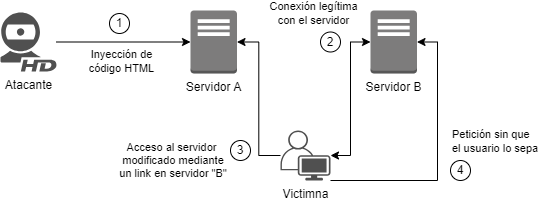
\includegraphics[width=0.9\linewidth]{fig/csrf.png}
    \caption{Ataque CSRF}
    \label{fig:csrf-attack}
\end{figure}


En el contexto de este proyecto, para mitigar este riesgo, se implementó medidas de seguridad como tokens CSRF. Estos tokens actúan como códigos secretos que deben incluirse en cada solicitud que puede realizar cambios en el estado del servidor (POST, PATCH, PUT, DELETE) y son verificados por el servidor para garantizar la legitimidad de la solicitud, evitando así que se realicen acciones no autorizadas en nombre del usuario.


\section{App Scripts}

``Apps Script es la única plataforma con bajo nivel de codificación que agiliza y facilita la compilación de soluciones empresariales que integran, automatizan y extienden Google Workspace.

Apps Script le permite compilar con HTML, CSS y JavaScript, sin que tenga que aprender un nuevo marco de trabajo exclusivo.''\cite{appscript}.

Apps Script ofrece una variedad de funcionalidades, permitiéndote realizar:

\begin{itemize}
\item Automatizaciones
\item Creación de complementos
\item Desarrollo de funciones personalizadas
\item Creación de Web Apps Script, entre otras opciones.
\end{itemize}

\subsection{Secciones de App Script}\label{sec:mt:app-script}

Dentro del archivo script creado con Google Apps Script, encontramos varias secciones que facilitan el desarrollo y la gestión de nuestros proyectos:

\begin{itemize}
\item \textbf{Información General:} Esta sección proporciona detalles sobre el script, la posibilidad de crear copias, visualizar el uso y los alcances utilizados.
\item \textbf{Editor de Código:} La sección principal donde programamos e implementamos nuestro código.

\item \textbf{Activadores:} Aquí creamos activadores o triggers basados en eventos o tiempo para ejecutar el script.

\item \textbf{Ejecuciones:} Esta sección muestra el historial de ejecuciones, logs y resultados obtenidos.

\item \textbf{Configuración:} Contiene configuraciones avanzadas para ajustar el comportamiento de nuestro script.
\end{itemize}


\subsection{Contexto del Proyecto}

En el marco de este proyecto, se empleó Google Apps Script como una solución integral para automatizar la carga de formularios en el sistema. Además, se utilizó para desarrollar plugins que mejoran la experiencia de gestión del usuario administrador mediante un menú y una interfaz gráfica intuitiva para la configuración eficiente de opciones.



\section{Web Sockets}
Según lo desarrollado en el artículo de IONOS \cite{sockets} se explican los siguientes conceptos.

Un \textbf{socket} es un mecanismo de comunicación que permite que dos procesos en diferentes máquinas o en la misma máquina se comuniquen entre sí. En términos simples, un socket proporciona una interfaz para la comunicación entre procesos.

Un \textbf{WebSocket} es un protocolo de comunicación bidireccional en tiempo real sobre un único socket TCP. A diferencia de HTTP, que sigue un modelo de solicitud-respuesta, los WebSockets permiten la comunicación en ambas direcciones en cualquier momento. La Figura \ref{fig:sockets} ilustra el concepto de Web Sockets.

El proceso típico para establecer una conexión WebSocket es:
\begin{itemize}
\item \textbf{Handshake (apretón de manos)}: El cliente envía una solicitud HTTP al servidor solicitando el establecimiento de una conexión WebSocket. Si el servidor acepta, se produce un “apretón de manos” y la conexión se actualiza a WebSocket.

\item \textbf{Comunicación bidireccional}: Después del “apretón de manos”, ambas partes pueden enviar y recibir datos de manera bidireccional en tiempo real a través del mismo socket.
\end{itemize}

\begin{figure}[h]
    \centering
    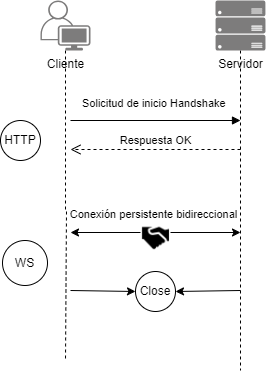
\includegraphics[width=0.5\linewidth]{fig/sockets.png}
    \caption{Web Sockets}
    \label{fig:sockets}
\end{figure}




\section{Patrón de Diseño Pub/Sub}\label{sec:pub-sub}

El patrón de diseño Publicador-Suscriptor, es una solución que permite a una aplicación comunicar eventos de manera asincrónica a múltiples consumidores interesados, evitando la necesidad de establecer una conexión directa entre los emisores y receptores.  La Figura \ref{fig:pub-sus} muestra una representación gráfica del patrón, un componente llamado ``publicador'' emite eventos a través de canales temáticos, y los "suscriptores" que están interesados en eventos específicos se registran en dichos canales.


\begin{figure}[h]
    \centering
    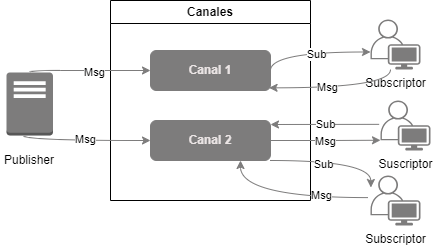
\includegraphics[width=0.8\linewidth]{fig/chanels.png}
    \caption{Publicador Suscriptor}
    \label{fig:pub-sus}
\end{figure}

En el contexto de este proyecto, se utiliza este patrón con el uso de web sockets en el sistema de notificaciones en tiempo real y actualizaciones de vistas.

\section{Docker Swarm}
\textbf{Docker} es una plataforma de código abierto diseñada para facilitar la creación, implementación y ejecución de aplicaciones en entornos aislados llamados "contenedores". Estos contenedores son unidades ligeras y portátiles que contienen todo lo necesario para que una aplicación se ejecute, incluidas bibliotecas, dependencias y código, de manera eficiente y coherente en cualquier entorno que admita Docker.

\textbf{Docker Swarm} es una herramienta de orquestación integrada en Docker que facilita la administración y escalabilidad de aplicaciones distribuidas que se ejecutan en contenedores Docker. Swarm permite la creación y administración de clústeres de Docker, donde múltiples nodos pueden trabajar juntos para proporcionar una plataforma robusta y escalable para la implementación de aplicaciones en contenedores.



\section{Normalización de la Base de Datos}

La normalización de una base de datos es un proceso esencial en el diseño de sistemas de gestión de bases de datos. 
Cabe destacar que cada forma normal depende de que se cumpla la forma normal anterior. Esto asegura que el proceso de normalización sea progresivo y que cada nivel proporcione una mayor reducción de redundancia y una mejora en la organización de los datos.
A continuación, se describen las formas normales principales:

\subsection{Primera Forma Normal (1FN)}

La 1FN elimina los grupos repetidos de las tablas individuales. En otras palabras, cada celda de la tabla debe contener un único valor atómico, evitando así la repetición de grupos de datos.

\subsection{Segunda Forma Normal (2FN)}

La 2FN establece que, si un atributo no forma parte de la clave primaria, debe proporcionar un hecho que dependa de la clave completa. Esto elimina dependencias parciales y contribuye a una mejor organización de los datos.

\subsection{Tercera Forma Normal (3FN)}

La 3FN va un paso más allá y elimina los campos que no dependen directamente de la clave primaria. Esto ayuda a asegurar que cada campo en una tabla contribuya únicamente a la información específica de esa clave.

\subsection{Forma Normal de Boyce-Codd (FNBC)}

La Forma Normal de Boyce-Codd (FNBC) es una extensión de la 3FN. Si no existen claves candidatas compuestas, una tabla se considera en FNBC. Sin embargo, si hay claves candidatas compuestas con un elemento común, puede no estar en FNBC, a menos que cada determinante en las dependencias funcionales sea una clave candidata.

\section{Propiedades ACID en Bases de Datos}

En el contexto de bases de datos, las propiedades ACID son fundamentales para garantizar la integridad y confiabilidad de las transacciones.

\begin{itemize}
  \item \textbf{Atomicidad (A):} Asegura que una transacción se realice de manera completa o no se realice en absoluto.

  \item \textbf{Consistencia (C):} Garantiza que la base de datos pase de un estado válido a otro válido después de que una transacción se haya completado.

  \item \textbf{Aislamiento (I):} Asegura que las transacciones en ejecución sean independientes entre sí, de modo que el resultado de una transacción no afecte el resultado de otras transacciones concurrentes.

  \item \textbf{Durabilidad (D):} Garantiza que una vez que una transacción se ha completado con éxito, sus cambios son permanentes y persisten incluso en caso de fallo del sistema.
\end{itemize}
